%%%%%%%%%%%%%%%%%%%%%%%%%%%%%%%%%%%%%%%%%
% Homework Assignment Article
% LaTeX Template
% Version 1.3.1 (ECL) (08/08/17)
%
% This template has been downloaded from:
% Overleaf
%
% Original author:
% Victor Zimmermann (zimmermann@cl.uni-heidelberg.de)
%
% License:
% CC BY-SA 4.0 (https://creativecommons.org/licenses/by-sa/4.0/)
%
%%%%%%%%%%%%%%%%%%%%%%%%%%%%%%%%%%%%%%%%%

%----------------------------------------------------------------------------------------

\documentclass[a4paper]{article} % Uses article class in A4 format

%----------------------------------------------------------------------------------------
%	FORMATTING
%----------------------------------------------------------------------------------------

\addtolength{\hoffset}{-2.25cm}
\addtolength{\textwidth}{4.5cm}
\addtolength{\voffset}{-3.25cm}
\addtolength{\textheight}{5cm}
\setlength{\parskip}{0pt}
\setlength{\parindent}{0in}

%----------------------------------------------------------------------------------------
%	PACKAGES AND OTHER DOCUMENT CONFIGURATIONS
%----------------------------------------------------------------------------------------

\usepackage{blindtext} % Package to generate dummy text
% \usepackage[style=numeric,sorting=none]{biblatex}
\usepackage{charter} % Use the Charter font
\usepackage[utf8]{inputenc} % Use UTF-8 encoding
\usepackage{microtype} % Slightly tweak font spacing for aesthetics

\usepackage[english]{babel} % Language hyphenation and typographical rules

\usepackage{amsthm, amsmath, amssymb} % Mathematical typesetting
\usepackage{float} % Improved interface for floating objects
\usepackage[final, colorlinks = true, 
            linkcolor = black, 
            citecolor = black]{hyperref} % For hyperlinks in the PDF
\usepackage{graphicx, multicol} % Enhanced support for graphics
\usepackage{xcolor} % Driver-independent color extensions
\usepackage{marvosym, wasysym} % More symbols
\usepackage{rotating} % Rotation tools
\usepackage{censor} % Facilities for controlling restricted text
\usepackage{listings, style/lstlisting} % Environment for non-formatted code, !uses style file!
\usepackage{pseudocode} % Environment for specifying algorithms in a natural way
\usepackage{style/avm} % Environment for f-structures, !uses style file!
\usepackage{booktabs} % Enhances quality of tables

\usepackage{tikz-qtree} % Easy tree drawing tool
\tikzset{every tree node/.style={align=center,anchor=north},
         level distance=2cm} % Configuration for q-trees
\usepackage{style/btree} % Configuration for b-trees and b+-trees, !uses style file!

% \usepackage[backend=biber,style=numeric,
            % sorting=nyt]{biblatex} % Complete reimplementation of bibliographic facilities
% \addbibresource{ecl.bib}
\usepackage{csquotes} % Context sensitive quotation facilities

\usepackage[yyyymmdd]{datetime} % Uses YEAR-MONTH-DAY format for dates
\renewcommand{\dateseparator}{-} % Sets dateseparator to '-'

\usepackage{fancyhdr} % Headers and footers
\pagestyle{fancy} % All pages have headers and footers
\fancyhead{}\renewcommand{\headrulewidth}{0pt} % Blank out the default header
\fancyfoot[L]{School of Computing, Macquarie University} % Custom footer text
\fancyfoot[C]{} % Custom footer text
\fancyfoot[R]{\thepage} % Custom footer text

\usepackage{comment}
\newcommand{\note}[1]{\marginpar{\scriptsize \textcolor{red}{#1}}} % Enables comments in red on margin

%----------------------------------------------------------------------------------------

\begin{document}

%----------------------------------------------------------------------------------------
%	TITLE SECTION
%----------------------------------------------------------------------------------------

\title{COMP3100 project report} % Article title
\fancyhead[C]{}
\hrule \medskip % Upper rule
\begin{minipage}{1\textwidth} % Center of title section
\centering 
\large % Title text size
Project report: Stage 1\\ % Assignment title and number
COMP3100 Distributed Systems, S2, 2022\\
\normalsize % Subtitle text size
SID: 46293175, Name: Quoc Huy Pham
%%%%\\ % Assignment subtitle
\end{minipage}
\medskip\hrule % Lower rule
\bigskip

%----------------------------------------------------------------------------------------
%	ARTICLE CONTENTS
%----------------------------------------------------------------------------------------
\section{Introduction}

This report focuses on designing and implementing a client-side simulator that acts as a simple job dispatcher using the TCP/IP protocol. The simulator works by contacting a virtual server simulator: \href{https://github.com/distsys-MQ/ds-sim}{ds-sim} \cite{ds-sim}, receiving jobs from the server-side simulator, and scheduling them using a Largest-Round-Robin (LRR) dispatcher/scheduler. LRR sends each job to a server of the largest type in a round-robin fashion, where the most significant server type is defined as the one with the biggest number of CPU cores. If there are two server types with the same biggest core count, use the first one.
\\This project is a minor part of a more significant project for unit COMP3100, in which students have to develop a functional client-side simulator for ds-sim that can utilise multiple job scheduling algorithms such as  First-Fit (FF), Best-Fit (BF) and Worst-Fit (WF).
\\The stage 1 project, which is what this report is written for, will focus on basic communication with \href{https://github.com/distsys-MQ/ds-sim}{ds-sim} \cite{ds-sim} and LRR task scheduling.

\section{System Overview}
\label{sec:section2}

This section covers a general overview of how the client communicates with the ds-server in \href{https://github.com/distsys-MQ/ds-sim}{ds-sim} \cite{ds-sim}. The interaction can be summarised as follow:

\begin{enumerate}
    \item Client establishes a connection with the ds-server through the required port.
    \item Client establishes handshaking with the ds-server.
    \item Client collects information about the server's statistics.
    \item Client collects information about jobs that are required to schedule.
    \item Client starts scheduling.
    \item Client terminates the connection to the server if task scheduling is done. 
\end{enumerate}

There are some constraints to this stage of the project to make sure Largest-Round-Robin scheduling is functional:

\begin{itemize}
    \item Jobs being scheduled are completely independent of each other.
    \item There will be no job type that requires more processing data compared to the biggest servers.
\end{itemize}

The below figure summarises the entire process:
\begin{figure}[h!]
    \centering
    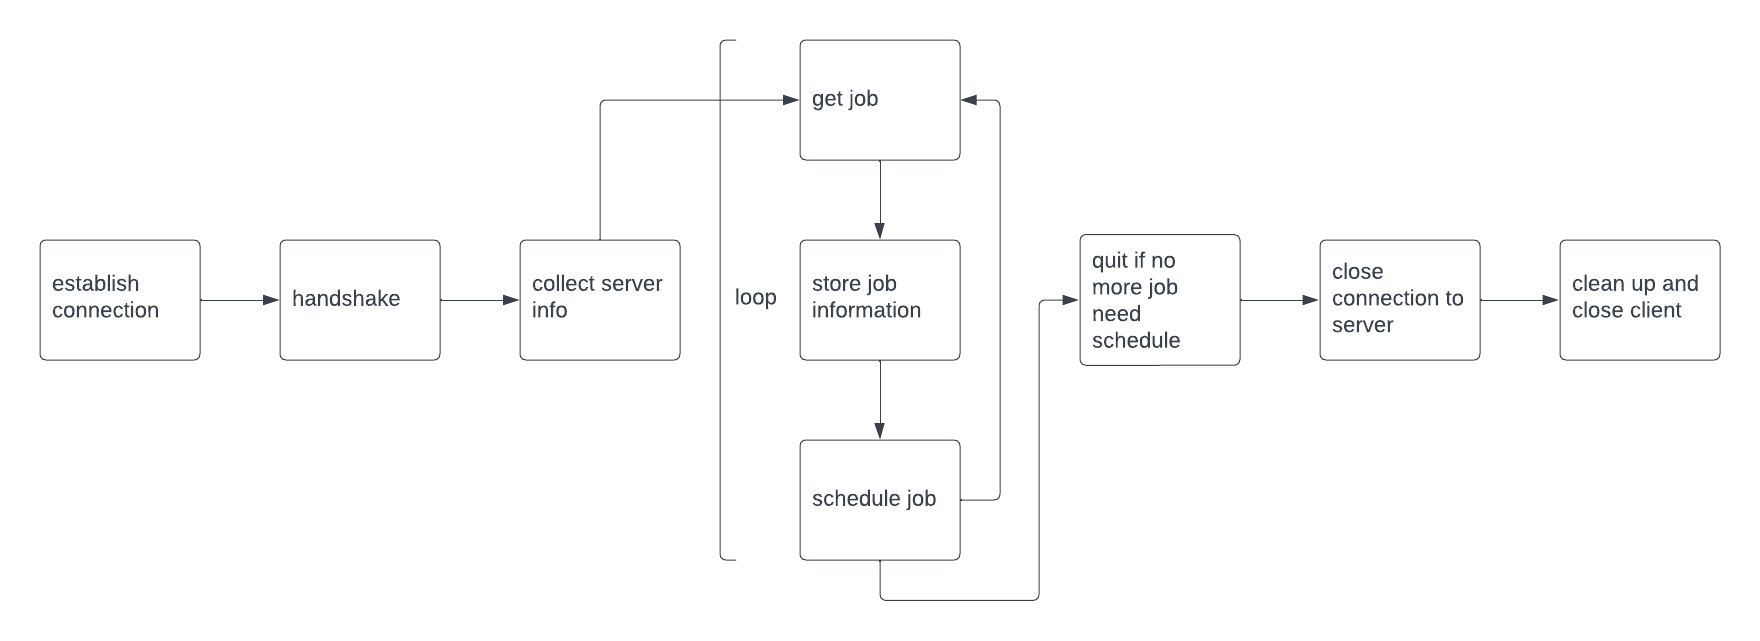
\includegraphics[scale = 0.25]{img/COMP3100 stage 1 diagram 1.png}
    \caption{client operation cycle}
    \label{fig:fig1}
\end{figure}\\

\section{Design}
\label{sec:section3}
\subsection{Design Philosophy}
The Philosophy for this client design is automatisation. All operations executed by the client are automatic; from establishing the connection to the server and handshaking up to job scheduling operating without manual input.
\\Regarding the coding style, it was written with modularity in mind. Although not perfect, it will allow certain functionalities to be independent of others, which should help maintainability and upgradability in the future (stage 2 of the project).

\subsection{Constraints and considerations}
Regarding the programming aspect of this project, there were some constraints that sightly affected decisions being made. During stage 1, LRR is the only schedule algorithm required. This constraint helped the development process simpler because only one direction was needed to achieve the requirement. although with modularity in mind, for later stages, implementing multiple scheduling algorithms can be troublesome with the current codebase. Further refactoring and cleaning are being considered because it can help ease the future development of the project. 
\\The application of LRR also creates some constraints on the way the client handles job scheduling in the future. At the moment, the client can only schedule jobs to servers consecutively. This works well with LRR scheduling, but with other scheduling algorithms where parallelism is required e.g handling multiple jobs to a server that can do more than one job, this can create problems. The only consideration available for this constraint is either to create either an algorithm that can execute job scheduling parallelism dynamically or a switch to change between different job scheduling.
\subsection{Server and client simulator}
The server reads a configuration file that defines the properties of servers and jobs, which are dynamically generated. When a client connects and completes the handshaking, the server generates a job or information about the job queue or server statuses. This process continues for the duration of the simulation.
\\The client executes based on the replies generated from the server. It starts with a connection to the server and receives information about the available servers and the current job to be scheduled. Based on the available servers and their properties, the client makes a scheduling decision. It then requests a new job to process, and the cycle continues until the server responds with 'NONE', meaning that there are no more jobs to be completed. After that, the client closes the connection, cleans up its input/output and ends the simulation. 

\begin{figure}[h!]
    \centering
    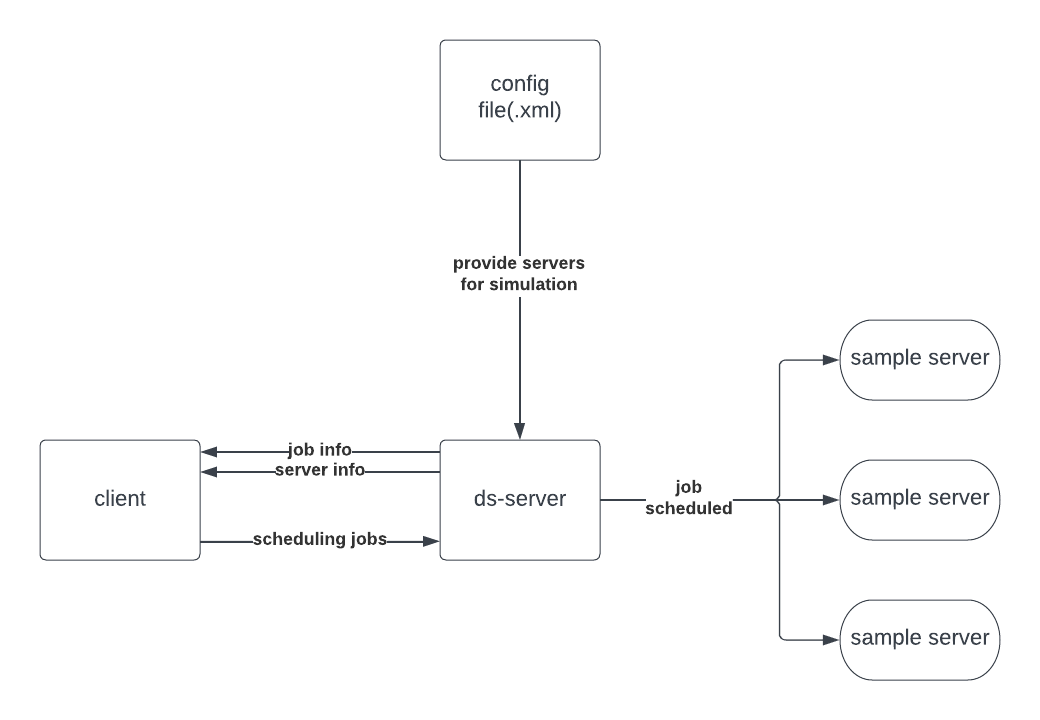
\includegraphics[scale = 0.3]{img/COMP3100 stage 1 diagram 2.png}
    \caption{client/ds-server simulator visualised}
    \label{fig:fig2}
\end{figure}\\

\section{Implementation}

The server was written and compile with java with Open JDK version 17 and in Ubuntu 22.10 Operating system. The server has four methods:
\begin{itemize}
    \item main() method: main method of the client, responsible for executing other methods, collect and store data and scheduling jobs.
    \item handshake(): responsible for executing handshaking to ds-server.
    \item receivedFromServer(): manage messages sent by ds-client.
    \item sendToServer(): send messages to ds-server.
\end{itemize}

\subsection{handshake() method}
The handshake() method performs the initial handshaking with the ds-server. It sends three messages to the server in the following order:
\begin{itemize}
    \item HELO message
    \item AUTH message with the current user's username as the argument
    \item REDY message
\end{itemize}
After sending each message, it waits for a response from the server and stores the received message in the serverInput variable through receivedFromServer() method.
\subsection{receivedFromServer() method}
The receivedFromServer() method is used to read and store messages sent by the server to the client. It reads a line of text from the input stream of the client's socket, stores the text in the serverInput String, and prints the received message to the console for debugging. This method is used to receive messages from the server throughout the program, such as receiving information about the available servers.
\subsection{sendToServer() method}
The sendToServer() method sends a message to the server over the output stream by writing the message as a byte array to the stream. Byte array was used instead of UTF due to ds-server only supporting ASCII single-byte encoding. The message is also printed to the console for debugging purposes. The method takes a string as input, which is the message to be sent to the server. The method also add an EOF condition (end of file) before sending the string so ds-server can read the stream properly.
\subsection{main() method}
The main() method executes all client functionalities, which includes previously mentioned methods, finds the biggest server type and does job scheduling. This method requires more refactoring. The method does the following task in order:

\begin{enumerate}
    \item The main() method establishes a connection to the ds-server at localhost and port 50000 using a Socket object. It also initialises the input and output streams for sending and receiving messages to and from the server.

    \item It calls the handshake() method to establish communication with the ds-server by sending HELO, AUTH, and REDY messages to the server and waiting for a response.

    \item If the server sends a message indicating that there are jobs available for scheduling, the main() method processes the job information, sends a GETS message to the ds-server to request information about available servers, and then stores the data received from the ds-server about available servers.

    \item The main() method then enters a loop to schedule jobs with LRR job scheduling algorithm. It sends SCHD messages to the server to schedule jobs on the largest available server and waits for a response from the server before sending another REDY message to the server to request another job.

    \item Once the ds-server responds with "NONE" indicating that there are no more jobs to be scheduled, the main() method sends a QUIT message to the server to terminate the connection, closes the input and output streams and the Socket object.
\end{enumerate}
\subsubsection{Conditions to find the biggest server type}
It starts by comparing the number of available cores on the current server with the highest number of available cores found so far (biggestSeverCoreCount). If the current server has more available cores than the previous server, it replaces the previous server as the biggest server and adds the current server's ID to the list of eligible servers. If the current server has fewer available cores than the previous server, the loop continues to the next server without making any changes. If the current server has the same number of available cores as the previous server, it checks if they are the same server. If they are the same server, it adds the current server's ID to the list of eligible servers. If they are different servers, the loop continues to the next server. 
\\At the end of the loop, the list jobServerIDs contains the IDs of all eligible servers with the highest number of available cores. These filtering conditions may require refactoring because it is hard to read to an extent.
\subsubsection{Largest-Round-Robin }
LRR was implemented as follow:
\begin{enumerate}
    \item Changing serverInput into the initial job message stored at the beginning of main() 
    \item The loop starts with the stop condition being no job left to schedule ("NONE" sent by ds-server)
    \item Inside the loop, the code first splits the serverInput variable into an array of strings called params, and then parses the third element of the params array as an integer, which represents the job ID.
    \item If the serverInput variable contains the string "JOBN" (which it should), then the code schedules the job using the biggest server and server IDs obtained from the previous part of the code. The index variable is used to cycle through the available job server IDs, and if it reaches the end of the list, it resets back to 0.
    \item After scheduling the job, the code sends the "REDY" command to the server and depends on whether jobs are available to schedule or not. it starts another iteration of the loop.
\end{enumerate}
\subsection{Github link}
https://github.com/Fozzyishere/COMP3100.git
%----------------------------------------------------------------------------------------
%	REFERENCE LIST
%----------------------------------------------------------------------------------------
\bibliographystyle{ieeetr}
\bibliography{comp3100project}
% \printbibliography
\bibitem[]{}
%----------------------------------------------------------------------------------------

\end{document}
